
Para que o um veículo aéreo não tripulado funcione de forma completa, é necessário definir um sistema de fornecimento de energia eficiente, para que o mesmo consiga suprir todas as necessidades dos sistemas que terão funções de controle e comando.

\subsubsection{Bateria}

Uma bateria é um dispositivo capaz de armazenar energia química e transformá-la em energia elétrica. A bateria é entendida geralmente como algo que possui duas ou mais células elétricas individuais, e existem dois tipos básicos de células: primária e secundária \cite{gibbs}. As primárias, identificadas como células normais, não são recarregáveis e devem ser descartadas quando esgotadas. Já as secundárias, são recarregáveis, como a bateria do tipo polímero de lítio, que foi a escolhida para atuar neste projeto, e será apresentada posteriormente. 

Para determinar a escolha da bateria utilizada em qualquer projeto, é importante fazer a análise  da energia armazenada na bateria e a variação de descarga ao ser utilizada, e para calcular a energia armazenada, deve-se conhecer a tensão (V) e sua capacidade de descarga de corrente no tempo (Ah), utilizando a equação a seguir: \cite{peixoto}

$Energia(Wh)= Tensão(V)*Capacidade(Ah)$

Onde tensão ou diferença de potencial (DDP), é a diferença de potencial elétrico entre dois pontos ou a diferença em energia elétrica potencial por unidade de carga elétrica entre dois pontos, e sua unidade de medida é o Volt. E Capacidade (amp-hora ou mA-h) é a transferência de carga elétrica através de uma corrente estável de um ampere no período de uma hora \cite{gibbs}.

Além disso, deve-se também conhecer a densidade de energia (relação entre quantidade de energia por unidade de massa ou Volume), Resistência interna, voltagem, peso, viabilidade econômica e disponibilidade no mercado.


\subsubsection{Atuação do circuito na bateria}

O diagrama da figura \ref{fig:esquemabateria}, demonstra funciona o sistema de alimentação do circuito elétrico do VANT. É possível identificar a bateria principal (batt), ela é ligada a porta de alimentação do modulo de potência 3DR Pixhawk, que foi usado pois a bateria que está sendo usada necessita devido suas especificações. Posteriormente tudo é ligado a uma placa de distribuição de potência (PDB), onde ela é a responsável para suprir a necessidade do sistema, ela que alimentará a controladora Pixhawk com seus periféricos e mandará energia suficiente para suprir a corrente exigida dos escs para o funcionamento dos motores. Por segurança, há uma segunda fonte de alimentação, uma fonte de 5V (BEC), ela é para casos onde houver uma falha na fonte primária, dessa forma ela será automaticamente ativada para evitar possíveis falhas \cite{pix}.

\begin{figure}[H]
    \centering
	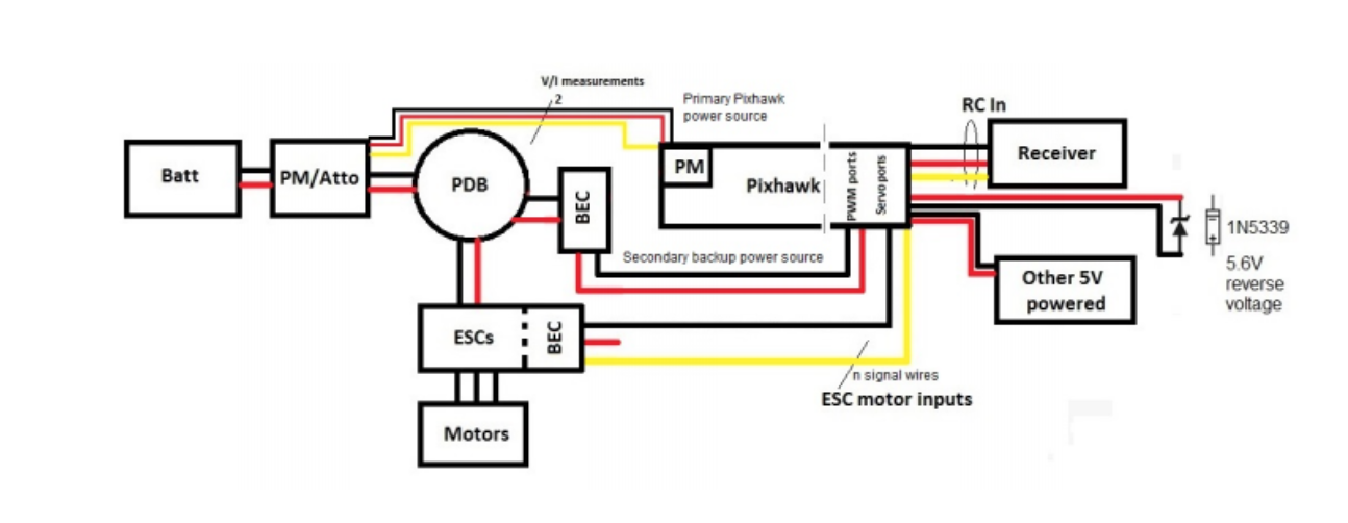
\includegraphics[keepaspectratio=true,scale=0.6]{figuras/esquemabateria.eps}
    \caption{Diagrama de blocos da bateria ligada ao controlador}
    \label{fig:esquemabateria}
\end{figure}


\subsubsection{Bateria de polímeros de Lítio (Li-Polymer)}

Baterias de polímeros de Lítio (LiPo) são aquelas que contem seus eletrólitos retidos em um polímero sólido, 
composta por várias células secundárias finas idênticas ligadas em paralelo, o que aumenta sua capacidade de 
descarga, sendo essencial que ela opere em uma faixa entre sua voltagem, não excedendo nem diminuindo muito, para perfeito funcionamento. \cite{gibbs}

As células de lítio-polímero são feitas de três componentes principais: um catodo (placa positiva), um anodo 
(placa negativa) e um separador. O catodo e o anodo são feitos principalmente de lítio, já o separador é feito 
de folhas rígidas de polímero banhadas em eletrólito. \cite{gibbs}

São flexíveis e oferecem leveza, já que não se faz necessário uma camada metálica externa como as baterias de 
Lítio-Íon, e podem ser facilmente moldadas para diversas aplicações. Também possuem uma resistência interna 
baixa que se adequa bem as altas taxas de descargas. \cite{costa}. Usada comercialmente desde 1999 as baterias 
de polímeros de Lítio possuem densidade de energia em torno de 100 e 130 Wh/kg, ou seja, quantidade de energia 
por volume relativamente alta, muito parecida com as baterias de Lítio-Íon. Com isso o fator mais importante para
análise é a tolerância para a sobrecarga, nas baterias de Lítio-polímero essa tolerância é maior, evitando um 
excesso de energia concentrado na bateria que ocasionaria a perda de rendimento ou até a perda total da bateria.
\cite{costa}

\subsubsubsection{Características bateria LiPo 6s}

O funcionamento básico da célula de bateria do tipo LiPo consiste em eletrólitos de sais de lítio retidos
em um polímero sólido com óxido de polietileno e o poliacrilonitrilo ao invés de solventes tornando-as
adaptáveis a diferentes formatos e permitindo altas taxas de descarga. A carga elétrica de uma bateria
corresponde a quantidade de carga, corrente, que pode ser fornecida por uma hora. 
A taxa de descarga corresponde ao quanto essa carga pode ser dissipada no mesmo intervalo de tempo. \cite{gibbs}

A escolha da bateria depende essencialmente dos motores aos quais a mesma irá alimentar, para que seja feita uma boa distribuição dessa tensão é necessário que seja utilizado um circuito eletrônico responsável para isso e pelo controle de velocidade do motor e demais funções (Zaccarelli,2012). Após diversas comparações com trabalhos de cunho técnico-científico, optou-se pela  LiPo 22.2 V, 22000mAh, pois a mesma oferecia maior tensão, capaz de alimentar a necessidade do sistema do drone como um todo, melhor relação peso quantidade de carga armazenada, possuir taxa de descarga adequada exigida pelo motor, além de aumentar a autonomia do sistema.

As baterias LiPo são classificadas em “S”, tal fator significa quantas baterias em série possui o conjunto. Cada célula Li-Po tem uma voltagem nominal de 3,7V, portanto multiplicamos o numero de “S” por 3,7V para saber a voltagem do pack.  A voltagem mínima das Li-Po é de 3,0V por célula, carregadas possuem 4,2V e podem ser armazenadas por longos períodos com 3,8V, na presente escolha, a bateria será composta por 6 células, totalizando os 22,2V de tensão nominal \cite{gibbs}.

Apesar de suas vantagens e de ser utilizada como um combustível e não como bateria, as baterias de LiPo estão propensas a sobrecarga durante o processo de carga devido a diversos fatores, o que pode ocasionar combustão Com isso, é necessária a utilização de carregadores adequados, ajuste correto de taxa de carga, utilização de balanceador de células evitando que a carga seja aplicada diretamente aos terminais principais do pack sem controle de voltagem, além de evitar o procedimento de carga ao identificar que as células do pack estão danificadas \cite{gibbs}.

Suas principais vantagens são: peso reduzido em comparação com as demais e fornecimento de altas correntes 
\cite{pinto}. Apesar de suas vantagens e de ser utilizada como um combustível e não como bateria,
as baterias de LiPo estão propensas a sobrecarga durante o processo de carga devido a diversos fatores, 
o que pode ocasionar combustão. Com isso, é necessária a utilização de carregadores adequados, ajuste correto 
de taxa de carga, utilização de balanceador de células evitando que a carga seja aplicada diretamente aos 
terminais principais do pack sem controle de voltagem, além de evitar o procedimento de carga ao identificar 
que as células do pack estão danificadas. \cite{gibbs}

\subsubsection{Análise de custo}
Considerando os requisitos estipulados no escopo do projeto, foram levantadas discussões e pesquisas que culminaram na escolha da tecnologia lítio polímero (LiPO) para utilização na parte da alimentação energética do Vant. Essa tecnologia se sobressaiu em relação a todas outras estudadas por ser baterias que apresentam baixo peso, alta tensão, além de sua capacidade de fornecer elevadas correntes ao circuito e já ser uma tecnologia amplamente utilizada no meio aeroespacial.

Durante a escolha da bateria foram analisadas várias empresas ao redor de todo o mundo, sendo elas:

\begin{itemize}
 
\item Gens Tattu (Americana)

\item Foxtech (Chinesa)

\item Max Amps (Americana)

\item Robokits (Indiana)

\item Dronera (Norueguesa)

\item Honcell (Chinesa)

\end{itemize}

A empresa fornecedora foi escolhida com base em diversos aspectos, os quais foram: impostos relativos a importação, facilidade de contato com os fabricantes, renome internacional da empresa, densidade energética da bateria além do custo da bateria.

A  Tattu foi a empresa escolhida como fornecedora da bateria.  Dentre os fatores que mais pesaram na escolha foram a proximidade em relação ao Brasil, a facilidade de comunicação com o fabricante e também a qualidade da bateria. Foi observado que mesmo nas diferentes áreas ao redor do mundo as baterias não apresentam uma grande variação em relação ao custo, o que também favoreceu a empresa americana visto que as taxas de importação são relativamente inferiores, sendo que as únicas baterias relativamente mais baratas eram aquelas com um peso bastante superior às outras.

As especificações da bateria escolhida, como mostradas na figura 42, levam como base a potência  necessária de vôo do VANT, que, por sua vez, está relacionada ao tempo de vôo e também ao seu peso. Serão  necessárias  apenas  uma  bateria com capacidade  de  22000 mAh,  o que  somaria aproximadamente 500 dólares ao custo do projeto, cerca de 1574 reais de acordo com as cotações  atuais. A figura 43 faz uma comparação de preço com outras baterias encontradas no mercado..


\begin{figure}[H]
    \centering
	
\includegraphics[keepaspectratio=true,scale=0.6]{figuras/baterialipo.eps}
    \caption{Bateria LiPO escolhida e suas especificações}
    \label{fig:baterialipo}
\end{figure}

\textbf{Tabela comparativa entre baterias}

\begin{figure}[H]
    \centering
	\includegraphics[keepaspectratio=true,scale=0.6]{figuras/tabelabateria.eps}
    \caption{Tabela comparativa de baterias.}
    \label{fig:tabelabateria}
\end{figure}


\subsubsection{Cálculo da autonomia e taxa de descarga do EmerVant}

Para o cálculo da autonomia de voo do EmerVant, baseamos em fórmulas sobre física e eletricidade, onde pudemos calcular a densidade da energia (wh/kg) através da tensão (V), capacidade (mA-h) e o peso da bateria(kg). 

Por seguinte, para o cálculo da autonomia, que é a duração em horas que funcionará a bateria sem recarga, considera-se que a densidade de energia da bateria que escolhemos para alimentar os motores do Drone é o que vai definir a autonomia de voo calculando a energia total armazenada na bateria,a potencia de saída, o tempo de uma hora, o empuxo especifico, empuxo total e energia total, necessária para manter o Drone voando por uma hora. Considerando que o peso total estimado do EmerVant é de 8389g, sendo:

\begin{itemize}
\item 2509g da bateria;
\item 2600g (8 bracos), onde 1 braço = 325g (Incluindo motor e hélice);
\item 1200g do desfibrilador;
\item 750 g do respirador;
\item 1330 do Peso Frame central (esqueleto);
\item 38g da placa controladora PIXHAWK.
\end{itemize}

Também foi calculada a taxa de descarga (mA) que encontra-se por regra, estandardizada relativamente à capacidade total de armazenamento da bateria e a um dado período de tempo. Sua vida útil, que é o período em que a bateria funciona em modo eficiente, será em média de 500-1000 vezes.

Considerando a tensão elétrica (V) de  22.2 V e a capacidade (amp-hora ou mA-h) de 22.000mA-h, temos que: 

\begin{equation}
Quantidade de energia = V*C => 22.2V * 22Ah = 488.4Wh
\end{equation}

Substituindo na fórmula da densidade de energia: 

\begin{equation}
Densidade de energia = \frac{quantidade de energia}{P(bateria)} => \frac{488,4wh}{2,509kg} = 194,65 Wh/g.
\end{equation}

O cálculo da autonomia foi baseado na fórmula $ET=\frac{TT}{TEt}$, onde é composta por:

\begin{itemize}
\item E (Energia total armazenada na bateria) - É a corrente que a bateria pode oferecer durante T = 1h.
\item P (Potência de saída) - É a corrente (Amperes) multiplicada pela tensão (Volts). Em fórmula P=I*V.
\item T (Tempo) - Para definição de parâmetros, é considerado 1 hora.
\item TE (Empuxo Específico) - Este parâmetro indica quantos gramas de empuxo são obtidos para cada Watt de potência entregue ao motor. Seleciona-se a pior condição para o motor do tipo(dada por tabela) que será de 7.69 g/W.
\item TT (Empuxo total) - Usa-se a média entre a potência para subida e descida, ou seja, considera-se o valor médio de potência para o Drone parado no ar. Sendo assim seu TT seria igual ao valor do Peso(8427N).  
\item ET (Energia total) - Energia necessária para manter o Drone voando por uma hora. 
\end{itemize}

Aplicando na fórmula, tem-se:

\begin{equation}
ET=\frac{TT}{TE*1h} => \frac{8427}{7.69*1h} = 1095,8 Wh.
\end{equation}

Portanto, a autonomia do Vant será determinada pela quantidade de energia contida na bateria dividida pela ET:

\begin{equation}
Autonomia = \frac{488,4Wh}{1095,8Wh *(minutos)} = 44 MINUTOS.
\end{equation}

Visto que o Vant terá consumo no motor, Esc, Sensores e controladores, a autonomia cairá, e por motivo de segurança, foi trocada a bateria de 16000 mAh para uma de com maior  tensão (Lipo 6s 22000 mAh), tentando manter a autonomia necessária para o trabalho do EmerVant (20 minutos). 

No caso da taxa de descarga (mA), onde usamos a fórmula C= I*T, onde:

\begin{itemize}
	\item C= taxa de descarga
	\item I= corrente
	\item T= período analizado
\end{itemize}

Aplicando na fórmula, obtém-se: 

\begin{equation}
C= 5,2A* 60 minutos = 312mA.
\end{equation}

\subsubsubsection{Recarga da bateria}

A carga de uma bateria é explicada de forma simples por um fenômeno químico-físico que está envolvido com a eletrólise. \cite{gibbs}

Entretanto, essa simplicidade não deve ser subestimada, pois existem detalhes nesse tipo de bateria (Lipo 6s) que precisam ser levados em consideração dependendo da sua forma de uso.

Para o recarregamento da bateria que alimentará o VANT, será utilizada uma plataforma de recarga que funcionará diretamente ligada à  central de energia da estação de controle e fornecerá a energia necessária para o recarregamento da bateria quando o VANT necessitar.

A plataforma funcionará a partir de cabos específicos que estarão ligados a central energética da estação de controle. Assim, toda vez que o VANT retornar para a central alguma pessoa capacitada conectará o mesmo à plataforma de recarga. Ao aviso de recarga da bateria do VANT, a pessoa encarregada pela central desconectará os cabos.

A bateria de polímero de Lítio caso esteja acima da temperatura normal na hora da recarga, deve ser levada para um local afastado e ventilado, para que sua temperatura normalize.A maioria dos acidentes com baterias ocorrem durante a recarga. A bateria de lítio polimerizado em comparação com as outras tem um baixo risco de acidente nesse requisito. \cite{gibbs}

As baterias de Lítio Polimerizado tem dois requerimentos em relação as suas células, primeiramente a carga deve ser limitada a um valor seguro e em segundo lugar, a voltagem da célula não deve nunca ultrapassar 4.20 Vpc (Volts por célula). \cite{gibbs}

O carregador Li-PO é um dispositivo limitador de tensão que é semelhante ao sistema de chumbo-ácido. A diferença está em uma tensão mais elevada por célula, tolerância de tensão mais apertado e a ausência de carga de flutuação em plena carga.

As baterias de polímero de Lítio não podem ser carregadas por qualquer tipo de carregador, portanto, o escolhido para atuar no sistema de recarga do EmerVant foi o carregador iMax B6 (figura \ref{fig:carregador1}), se adequa de uma forma que carrega e balanceia adequadamente vários tipos de bateria de lítio, tais como a utilizada neste projeto (LiPo 6s), Li-íon e a série de bateria LiFe.


 \begin{figure}[H]
    \centering
	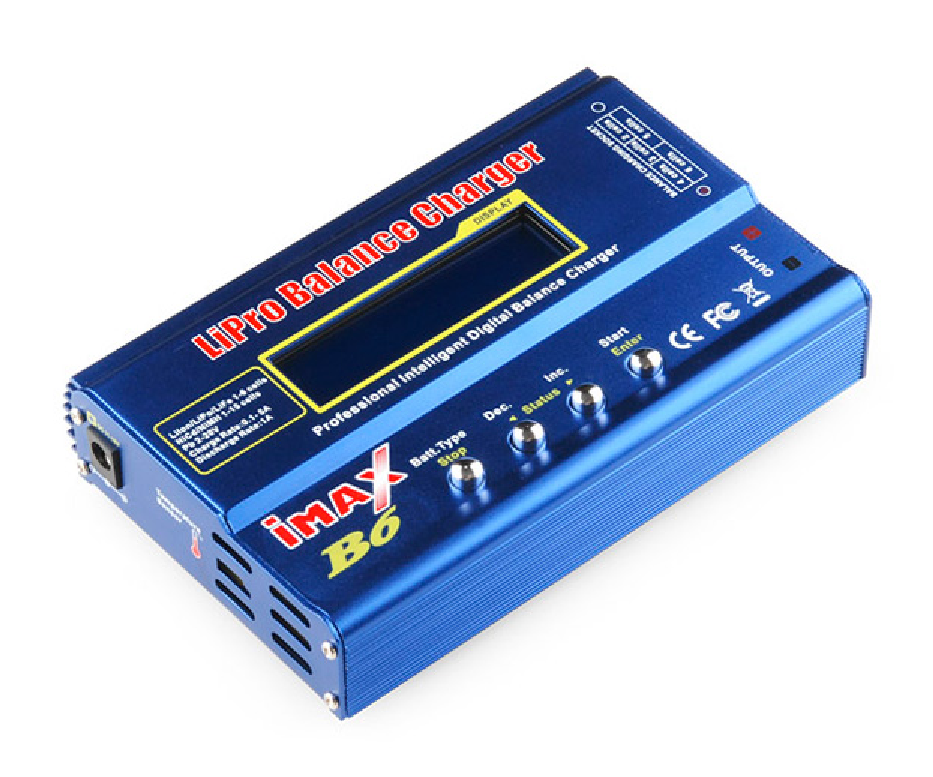
\includegraphics[keepaspectratio=true,scale=0.4]{figuras/carregador1.eps}
    \caption{Carregador iMax B6. Fonte: \cite{carregador1}}
    \label{fig:carregador1}
\end{figure}


Segundo o manual do usuário iMax B6 \cite{ibmax}, independente de qual seja a bateria de lítio usada, não será necessário se conectar a um balanceador externo para efetuar a carga de balanceamento, pois o mesmo emprega um balanceador de tensão de célula individual. Além disso, o B6 monitora e balanceia individualmente cada célula da bateria, onde apresenta uma mensagem de erro e é automaticamente interrompido caso apresente uma tensão anormal de qualquer célula individual. 

A figura a seguir mostra o menu do B6, que possui uma interface fácil de se interpretar, onde indica o carregamento e os ciclos em um processo simples, podendo ser feito de maneira rápida e precisa. O carregador não vem com a fonte de alimentação, porém contém um conector de entrada de CC que possui um \textit{plug} com garras tipo jacaré.

 \begin{figure}[H]
    \centering
	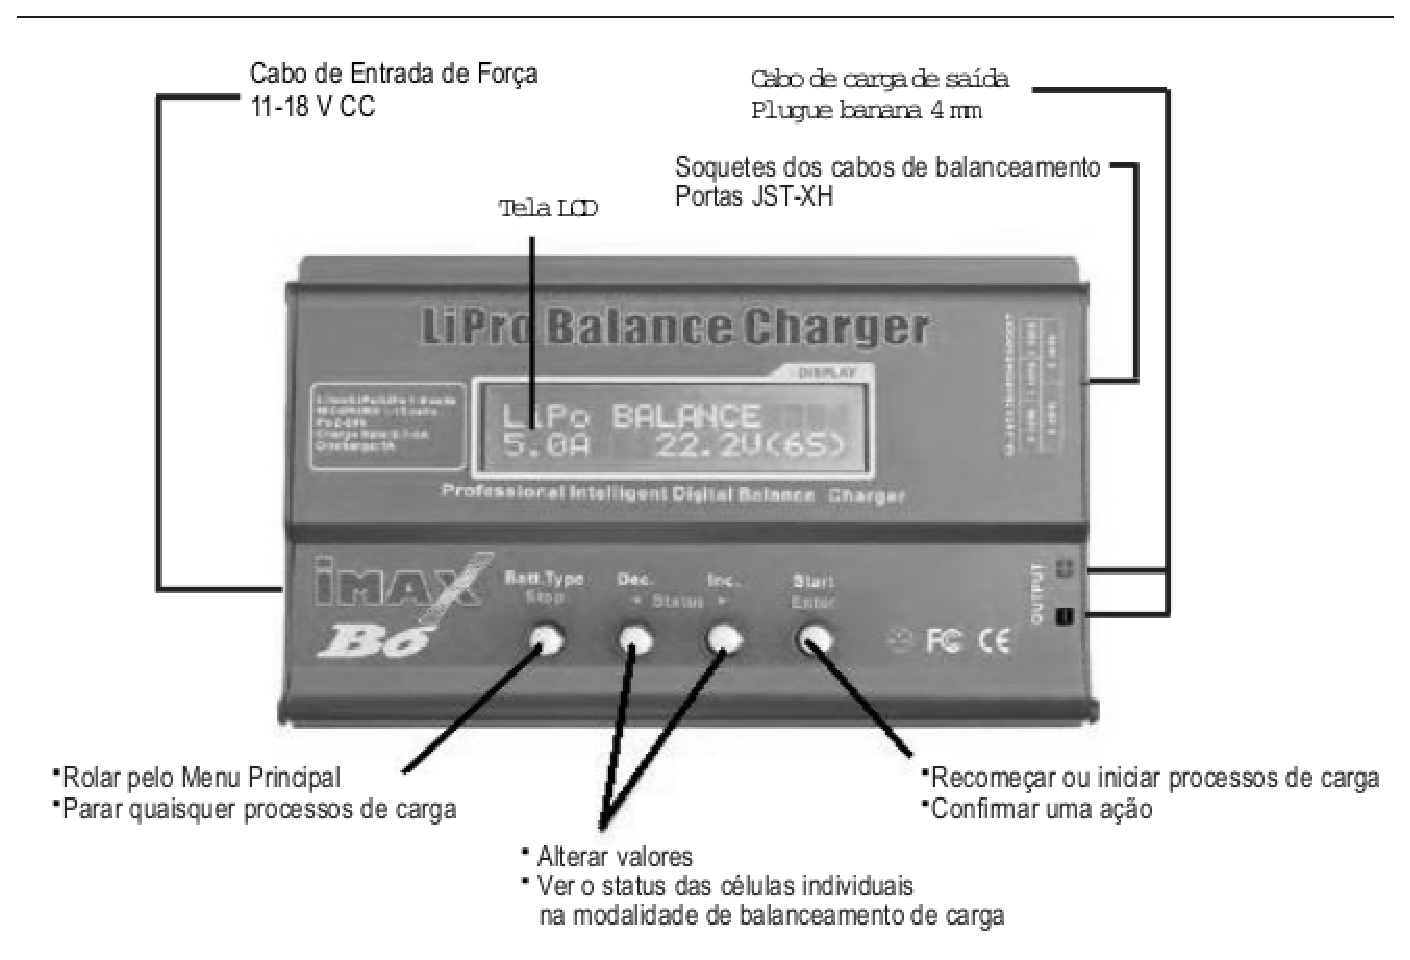
\includegraphics[keepaspectratio=true,scale=0.5]{figuras/manual.eps}
    \caption{Menu do iMax B6. Fonte: \cite{ibmax}}
\end{figure}
